\chapter{Results}
\label{result}

In this chapter, we report the results from all of our experiments and additional observations from the neural network's behavior.

\section{Enriching Encoder}
\label{result-enriching}

In this section, we report the results of our methods proposed in \cref{enriching}.

\subsection{Tree Distance and Traversal}

For the tree distance and tree traversal, it is shown that replacing the positional encoding or relative position with our proposed tree-related encodings does not help the translation.
All of the proposed methods are worse than the baselines.

As listed in \cref{tab:res-enriching}, on the test set, \transformerbase and \transformerrel achieved 36.66 and 37.02 BLEU, respectively, whereas \TreeTraversal, \TreeDistance max 5 and max 20 only got 35.80, 33.13 and 35.50 BLEU, in that order.
However, when the tree distance was combined with the positional encoding (\transformerbase) or the relative position (\transformerrel), it yielded better results than both baselines (37.49 and 37.55 vs. 36.66 and 37.02).
A similar gain was also seen in the case of tree traversal (37.80 vs. 37.02).

\begin{table}[t]
    \small
    \begin{center}
    \begin{tabular}{lcc}
        \textbf{Model}        	                            & \textbf{Dev}	& \textbf{Test}	\\
        \hline
        \transformerbase (base)    					        & 37.28 & 36.66 \\
        \transformerrel	(relative)				            & 37.23 & 37.02$^{\dag}$ \\
        \hline
        \TreeDistance, max 5				                & 35.47 & 33.13 \\
        \TreeDistance, max 20				                & 34.45 & 35.50 \\
        \TreeTraversal					                    & 35.21 & 35.80 \\
        (base) + \TreeDistance, max 5					    & 37.67 & 37.49$^{\ddag\blacktriangledown}$ \\
        % (base) + tree distance, max 20					    &  &  \\
        % (base) + tree traversal					        &  &  \\
        (relative) + \TreeDistance, max 20			        & 37.15 & 37.55$^{\ddag\blacktriangledown}$ \\
        (relative) + \TreeTraversal				            & 38.22 & \textbf{37.80}$^{\ddag\blacktriangledown}$ \\
        \hline
        (base) + \SpecPOS						& 36.97 & 36.65 \\
        (relative) + \SpecPOS			& 37.81 & 36.93$^{\dag}$ \\
        (base) + \SpecDep		& 37.53 &  37.72$^{\ddag\blacktriangledown}$ \\
        (relative) + \SpecDep		& 37.66 & \textbf{37.97}$^{\ddag\blacktriangledown}$  \\
    \end{tabular}
    \end{center}
    \caption[Enriching encoder results on \cs2en.]{Enriching encoder results on \cs2en. Statistical significance marked as $\dag$ ($p < 0.05$) and $\ddag$ ($p < 0.01$) when compared to \transformerbase and $\triangledown/\blacktriangledown$ when compared to \transformerrel.}
    \label{tab:res-enriching}
\end{table}

\subsection{Specialized Attention Head}

Also in \cref{tab:res-enriching}, for our second approach in the direction of enriching the encoder, the \SpecPOS model, whose one head in layer 0 was chosen to be dedicated as a specialized POS head, could not surpass the baselines (36.65 vs 36.66, 36.93 vs 37.02).

On the other hand, guiding this specialized attention head with dependency label embedding brought $+1.06$ BLEU over the \transformerbase (37.72 vs 36.66).
In addition, \SpecDep when combining with \transformerrel also achieved $+0.95$ BLEU over the \transformerrel (37.97 vs 37.02).

\section{Interpreting Self-Attention as Parse}
\label{result-promote}

This section presents the results of our joint models discussed in \cref{multitask}.

\subsection{Diagonal Parsing}
\label{result-promote-diagonal}

Before discussing the result of the parsing tasks (diagonal parsing and dependency parsing), we would like to note that a multi-task model usually requires much longer time to train compared to the single task model, e.g. twice the training time.
However, all of our multi-task models discussed in this section and the following sections were also trained for only 500,000 steps in order to prove our hypothesis that the Transformer already captures syntactic information.
The comparison of training time will be reported in \cref{result-speed}.

\cref{tab:res-translate-monoparse} reveals the result of our joint model which is capable of translating and parsing the source sentence to the diagonal matrix.
The diagonal parsing precision is, as expected, very high, ranging from 99.95\% to 99.99\% on the test set.
This joint model also outperformed the baseline in translation task with all its variants (BLEU scores vary from 37.47 to 38.14, compared to 36.66).

Moreover, these results form an observable pattern, in which the best result comes from the model which demands the linearized tree from the head on layer 0.
Demanding that structure at deeper layers still helps but BLEU scores decrease.
We believe a possible explanation for this pattern is because the diagonal matrix represents the relation between the preceding token and the current token.
This is a very simple sentence structure and serves as an additional positional information to the absolute position embeddings.
Therefore, the sooner the model is forced to recognize this positional information (via training the parsing task), the better it can learn to do translation.

\begin{table}[t]
\small
\centering
\vspace{2ex}
  \begin{tabular}{lcc|cc}
    &  \multicolumn{2}{c}{\textbf{BLEU}} & \multicolumn{2}{|c}{\textbf{Precision}} \\
    & \textbf{Dev} & \textbf{Test} & \textbf{Dev} & \textbf{Test} \\
    \hline
    \transformerbase & 37.28 & 36.66 & -- & -- \\
    \hline
    Syntax demanded from head on layer 0 & 38.68 & \textbf{38.14} & 99.97 & 99.96 \\
    Syntax demanded from head on layer 1 & 39.11 & 38.06 & 99.99 & \textbf{99.99} \\
    Syntax demanded from head on layer 2 & 37.85 & 37.85 & 99.98 & 99.98 \\
    Syntax demanded from head on layer 3 & 37.93 & 37.70 & 99.97 & 99.98 \\
    Syntax demanded from head on layer 4 & 37.68 & 37.47 & 99.98 & 99.96 \\
    Syntax demanded from head on layer 5 & 37.53 & 37.54 & 99.96 & 99.95 \\
  \end{tabular}
  \caption[\DiagonalParse's results in translation (BLEU) and diagonal parsing (precision) on \cs2en.]{\DiagonalParse's results in translation (BLEU) and diagonal parsing (precision) on \cs2en. All test BLEU improvements are statistically significant with $p<0.01$ when compared to the \transformerbase.}
  \label{tab:res-translate-monoparse}
\end{table}

\subsection{Dependency Parsing}
\label{result-promote-dependency}

Similarly to \cref{tab:res-translate-monoparse}, \cref{tab:res-translate-depparse} presents the results of our joint dependency parsing and translation model.

Let us recall the discussion in \cref{multitask-dep-parsing} that the choice of the head from one layer which will serve as the dependency parse is arbitrary.
However, selecting the layer matters.
In the \transformer's encoder as used in our experiments, there are six multi-head attention layers.
\cref{tab:res-translate-depparse} shows the results of both tasks when different layers in the encoder were chosen to dedicate one of their self-attention heads to serve as the dependency matrix.

It is apparent from \cref{tab:res-translate-depparse} that layer 0 (the first layer) was a too shallow layer to demand the syntax from.
Demanding dependency syntax from this layer yielded undesirable results in both translation and parsing task.
The BLEU score of 36.60 is no improvement over the baseline (36.66), while the UAS is at least 8\% lower than other variants of the same model.
We believe this result can be attributed to the assumption that the self-attention mechanism at this layer can only handle input word embeddings, which perhaps tend to concern more about lexical meaning than syntax.
Therefore, it could not capture the complex dependency syntax, which is not as simple as the diagonal syntax mentioned in the previous section.
On the other hand, layer 1 performed well on the parsing task (90.78\%), and brought the best improvement to the translation task (38.01).
The translation performance seems to be decreasing with deeper layers as well (38.01 - 37.87 - 37.67 - 37.60), as we already observed in the diagonal parsing.
The reason, from our point of view, is also similar.
The dependency syntax should be introduced to the model early enough in order to encourage better attention.
At later stages, surface syntax becomes less relevant as the model builds its internal representation.
Demanding syntactic interpretation from the deeper layers thus needlessly consumes the model capacity.

The performance on the dependency parsing task is shown to behave in the opposite direction.
The UAS values in \cref{tab:res-translate-depparse} are increasing from the shallower to the deeper layer (82.85 - 90.78 - 91.18 - 91.43 - 91.56).
The highest UAS was achieved when the syntax is demanded from layer 4, while the model was still able to maintain a good translation performance.
This pattern could suggest that when reaching to the deeper layers, the encoder has already learned a good representation for each token.
By good, we mean that the relevant information from other tokens and the relation between those and the current token have been all brought together by the shallower layers.
Therefore, at these deeper layers, the model can infer the dependency syntax easier and better.

\begin{table}[t]
\small
\centering
\vspace{2ex}
  \begin{tabular}{lcc|cc}
    &  \multicolumn{2}{c}{\textbf{BLEU}} & \multicolumn{2}{|c}{\textbf{UAS}} \\
    & \textbf{Dev} & \textbf{Test} & \textbf{Dev} & \textbf{Test} \\
    \hline
    \transformerbase & 37.28 & 36.66 & -- & -- \\
    \hline
    Syntax demanded from head on layer 0 & 36.95 & 36.60 & 81.39 & 82.85 \\
    Syntax demanded from head on layer 1 & 38.51 & \textbf{38.01} & 90.17 & 90.78 \\
    Syntax demanded from head on layer 2 & 38.50 & 37.87 & 91.31 & 91.18 \\
    Syntax demanded from head on layer 3 & 38.37 & 37.67 & 91.43 & 91.43 \\
    Syntax demanded from head on layer 4 & 37.86 & 37.60 & 91.65 & \textbf{91.56} \\
    Syntax demanded from head on layer 5 & 37.63 & 37.67 & 91.44 & 91.46 \\
  \end{tabular}
  \caption[\DepParse's results in translation (BLEU) and dependency parsing (UAS) on automatically annotated data (\cs2en).]{\DepParse's results in translation (BLEU) and dependency parsing (UAS) on automatically annotated data (\cs2en). All test BLEU gains, except for layer 0, are statistically significant with $p<0.01$ when compared to \transformerbase.}
  \label{tab:res-translate-depparse}
\end{table}

It is important to remind the reader that the parsing results reported up to this moment were computed against the automatic parses of the parallel corpus.
To have a better sense of how our models perform on the gold-annotated dataset, we tested our models with the PDT test set for Czech.
The referential parser we used to compare against was from the winner of CoNLL Shared Task 2007 \citep{connl2007}, the latest available evaluation on the same dataset.

In addition to the PDT, we wanted to measure the performance on the new annotation convention --- the Universal Dependencies 2.0.
For this, we employed our additional dataset \de2cs.
As discussed in \cref{dataexp-data}, this dataset includes the source trees generated by UDPipe.
Therefore, we selected UDPipe to be the referential parser for this dataset.

\cref{multidec-results} presents the results, in which our proposed
model outperformed the baseline in the translation task on both dataset (14.27 vs. 13.96 and 38.01 vs. 36.66).

\begin{table}[t]
    \small
    \begin{center}
    \begin{tabular}{lcc}
        \textbf{Model}        	& \textbf{\de2cs}	& \textbf{\cs2en}	\\
        \hline
        \transformerbase    & 13.96	&  36.66 \\
        \DepParse		& 14.27$^\dag$	&  38.01$^\ddag$ \\
    \end{tabular}
    \end{center}
    \caption[BLEU scores on test sets for translation task.]{BLEU scores on test sets for translation task. Statistical significance marked as $\dag$ ($p < 0.05$) and $\ddag$ ($p < 0.01$) when compared to \transformerbase.}
    \label{multidec-results}
\end{table}

When evaluated on the gold-annotated test sets, \cref{multidec-results-parse} shows that our model achieved a better result in German (de - 81.23 vs. 74.27), but worse in Czech (cs - 82.53 vs. 86.28).
A possible excuse is that our model was trained using automatic treebanks, not the gold-annotated ones.
We expect that the model could perform better after fine-tuning with the gold-annotated treebanks but leave this for future work.

\begin{table}[t]
    \small
    \begin{center}
    \begin{tabular}{lcc}
    \textbf{Model}        	& \textbf{de}	& \textbf{cs}	\\
    \hline
    % Stanford \citep{dozat-qi-manning:2017:K17-3} & 84.10 & -- \\
    UDPipe 1.2 (de) 		& 74.27 & -- \\ % UAS: 74.15, LAS: 68.61 in CoNLL Shared task 2017
    Nakagawa (2007) 		& -- &  86.28 \\
    \DepParse			& 81.23 	&  82.53 \\
    \end{tabular}
    \end{center}
    \caption{UAS on the gold-annotated test sets for parsing task.}
    \label{multidec-results-parse}
\end{table}

\subsection{Self-Attention Analysis}
\label{result-promote-analysis}

\begin{figure}[t]
	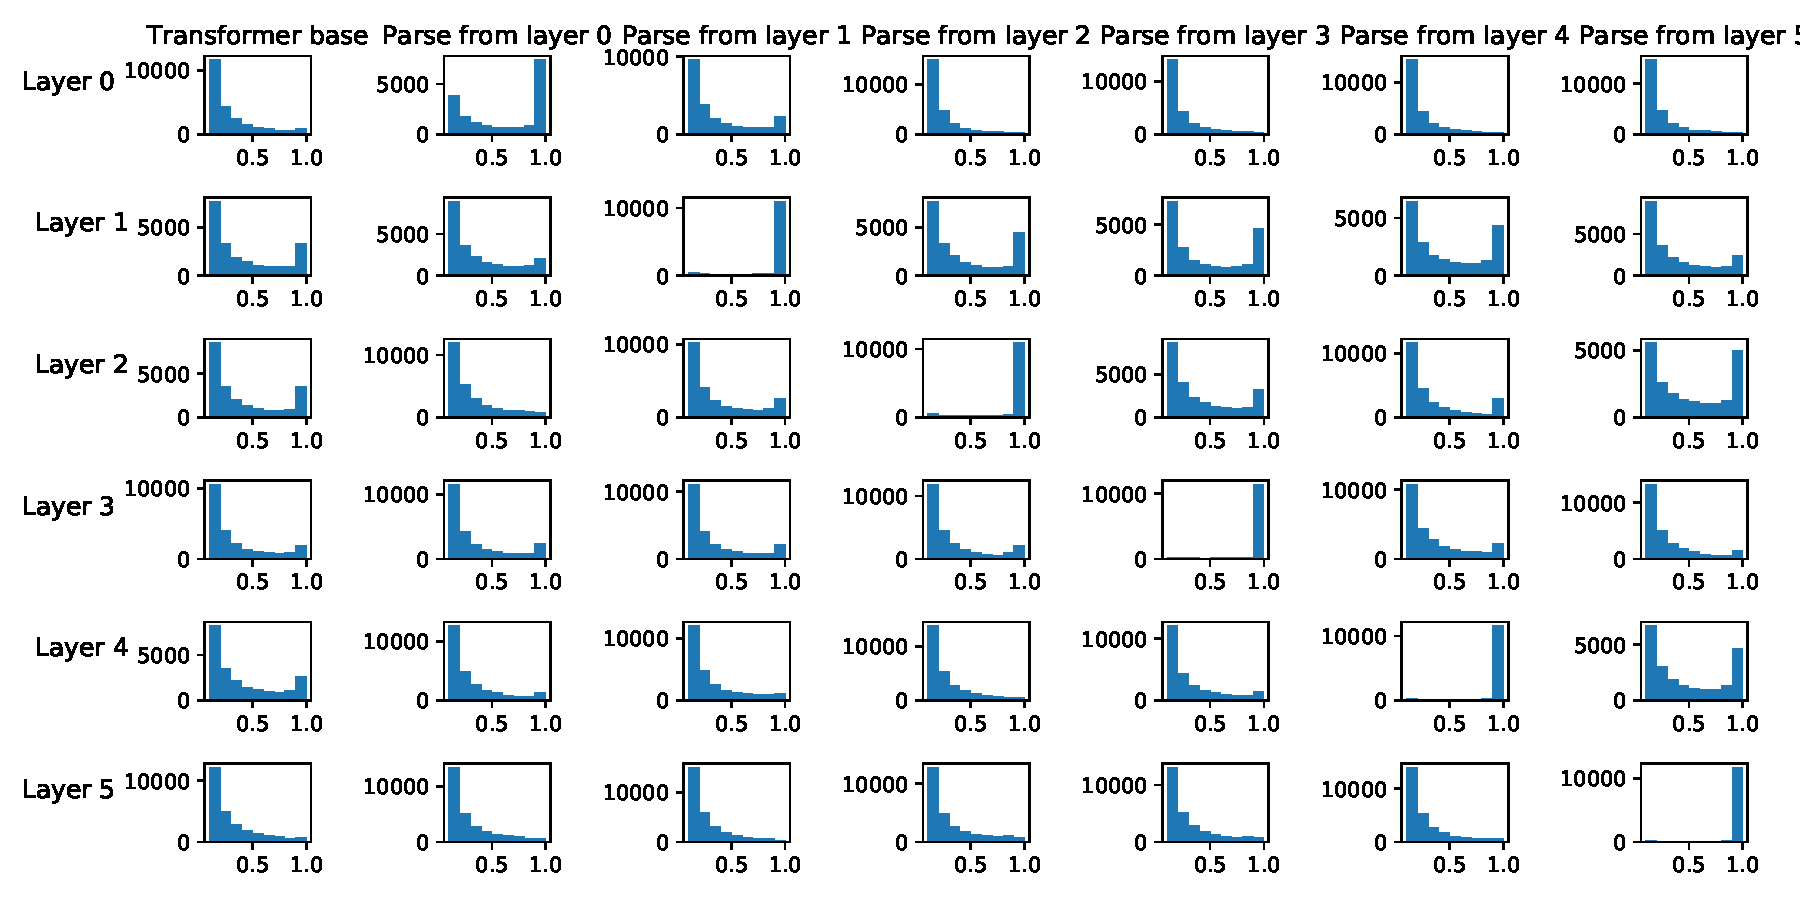
\includegraphics[width=\textwidth]{img/att_dist}
    \caption{Histogram of normalized self-attention weights for each layers (all 8 heads) in the encoder.}
    \label{fig:att_dist}
\end{figure}

In this section, we further analyze self-attention layers of the \DepParse and \DiagonalParse's encoders in the hope of a better understanding of the neural network we built.

Figure \ref{fig:att_dist} presents the behavior of self-attention mechanism in each layer of our model that jointly translates and proposes dependency edges.
In the figure, while each column represents one variant of our proposed model (except the first column which is the \transformerbase), each row ``Layer $i$" represents the $(i+1)$-th layer in that model.
The histograms of self-attention weights were computed after concatenating attention weights from all heads on that layer, and for the first 100 sentences in the \cs2en test set.
In addition, the bin $[0.0,0.1)$ has been removed for better visibility because most of the self-attention weights actually fell into this trivial bin.

As can be seen from the figure, the charts in the diagonal stand out, suggesting that the chosen layers have very sharp attention distributions, i.e. each head in the layer attends to only one or two other positions in the previous layer.
This behavior exists in all our multi-task models, except the ``Syntax demanded from head on layer 0".
As mentioned in \cref{result-promote-dependency}, this particular model performed badly on both tasks.
Our hypothesis is that this sharpness of attention due to our restricted self-attention helped the model to perform better.

One could argue that this sharp attention is expected for the head trained to produce syntactic tree.
The interesting observation is that \emph{all} heads in the respective layer also follow this pattern, as revealed in \cref{fig:att_dist_4}.

In \cref{fig:att_dist_4}, the histograms are computed separately for each head on layer 4 of the model where syntax was demanded from layer 4 (the bin $[0.0,0.1)$ was also removed from the plot).
For \DepParse (\cref{fig:att_dist_4_dep}), it is clear that not only the chosen head, but other heads in the same layer also have the sharp attention distribution.
A similar pattern can also be observed in the case of \DiagonalParse (\cref{fig:att_dist_4_mono}).
We believe the reason for this behavior lies in the concatenation and layer normalization after each multi-head attention layer.
The layer normalization over all heads may introduce the sharpness from the chosen head to other heads in the same layer.
We hypothesize that this caused a regularization in the network, which lead to our better performance in translation task.
However, in the scope of this thesis, the identification of the exact reason is left for future work.

\begin{figure}[t]
    \centering
    \begin{subfigure}[b]{\textwidth}
	    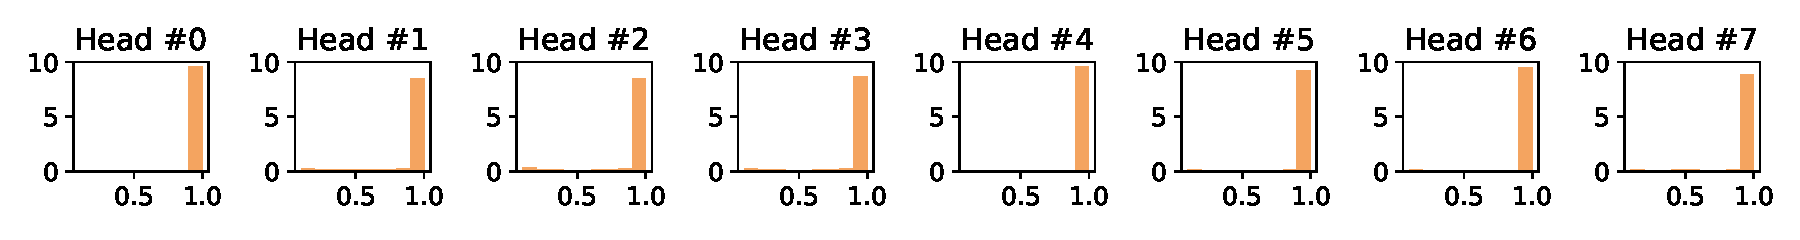
\includegraphics[width=\textwidth]{img/att_dist_4.pdf}
        \caption{\DepParse model.}
        \label{fig:att_dist_4_dep}
    \end{subfigure}
    \par\medskip
    \begin{subfigure}[b]{\textwidth}
	    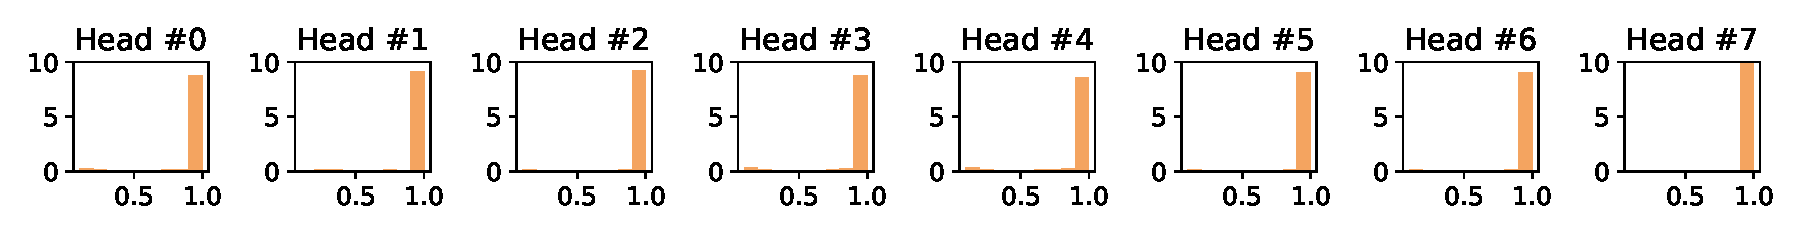
\includegraphics[width=\textwidth]{img/mono_att_dist_4.pdf}
        \caption{\DiagonalParse model.}
        \label{fig:att_dist_4_mono}
    \end{subfigure}
    \caption{Histogram of self-attention weights for each head in layer 4 when demanding the parse tree from layer 4.}
    \label{fig:att_dist_4}
\end{figure}

\cref{fig:att-from4} illustrates the sharpness studied above perhaps in a more intuitive way, by visualizing the attention weights for our sample sentence.
The model generated this sample is \DepParse that translates and produces dependency from one head on layer 4.
It is obvious that the attention edges on layer 4 are sharper, each token concentrates on a smaller number of tokens in the sentence.
On the other layers, each token attends to nearly all other tokens in the sentence, with a smaller weight for each attention edge.

\begin{figure}[t]
    \centering
    \begin{subfigure}[b]{0.9\textwidth}
        \centering
	    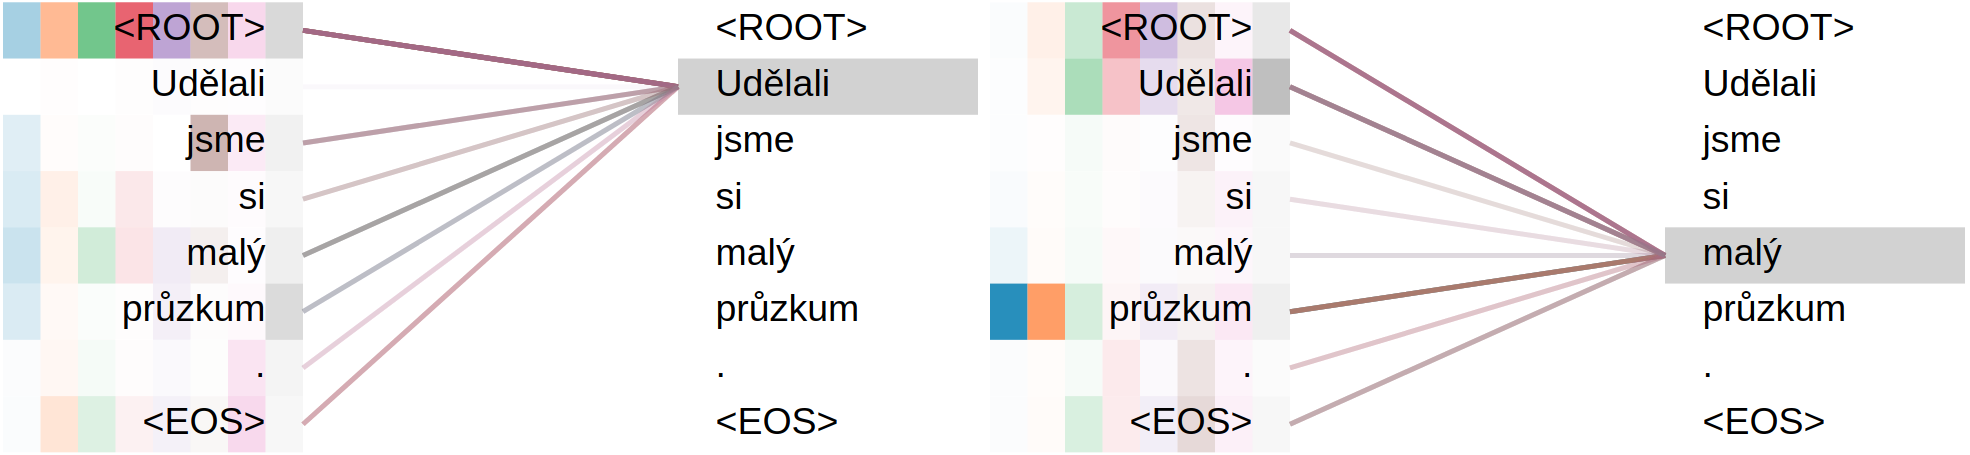
\includegraphics[width=\textwidth]{img/att-from4-l0.png}
        \caption{Layer 0}
    \end{subfigure}
    \par\medskip
    \begin{subfigure}[b]{0.9\textwidth}
        \centering
	    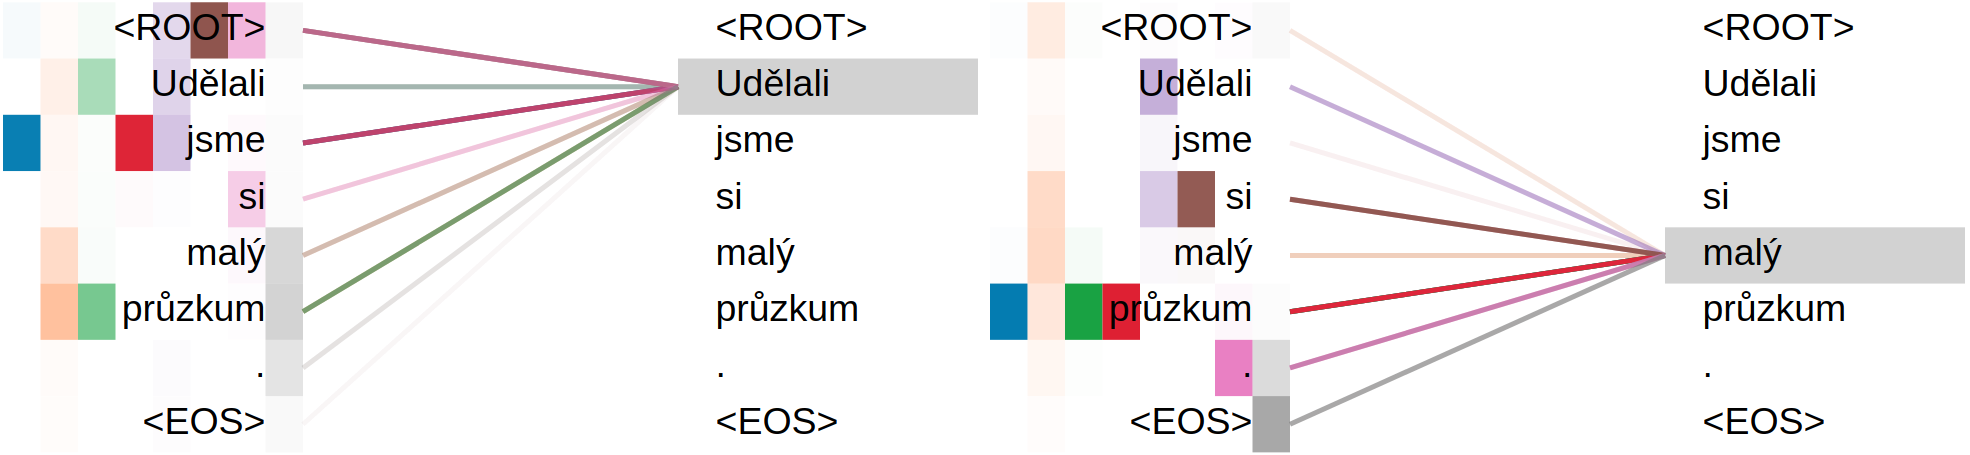
\includegraphics[width=\textwidth]{img/att-from4-l1.png}
        \caption{Layer 1}
    \end{subfigure}
    \par\medskip
    \begin{subfigure}[b]{0.9\textwidth}
        \centering
	    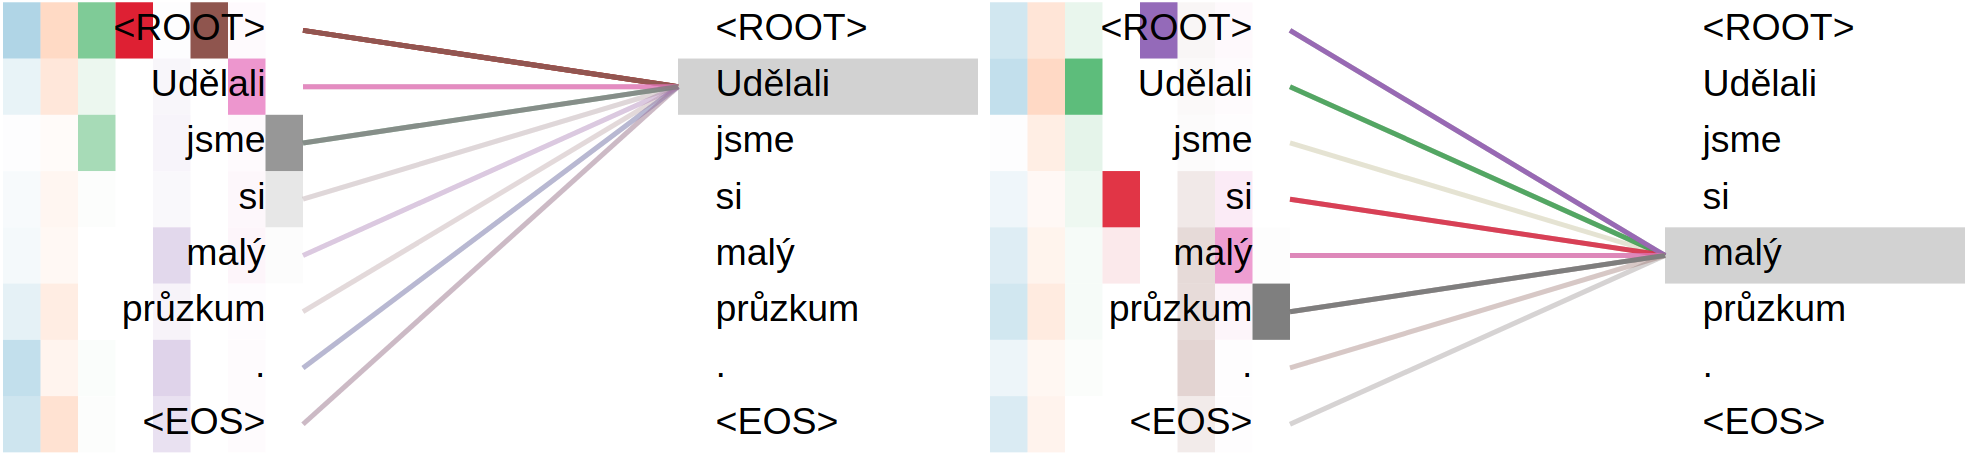
\includegraphics[width=\textwidth]{img/att-from4-l2.png}
        \caption{Layer 2}
    \end{subfigure}
    \par\medskip
    \begin{subfigure}[b]{0.9\textwidth}
        \centering
	    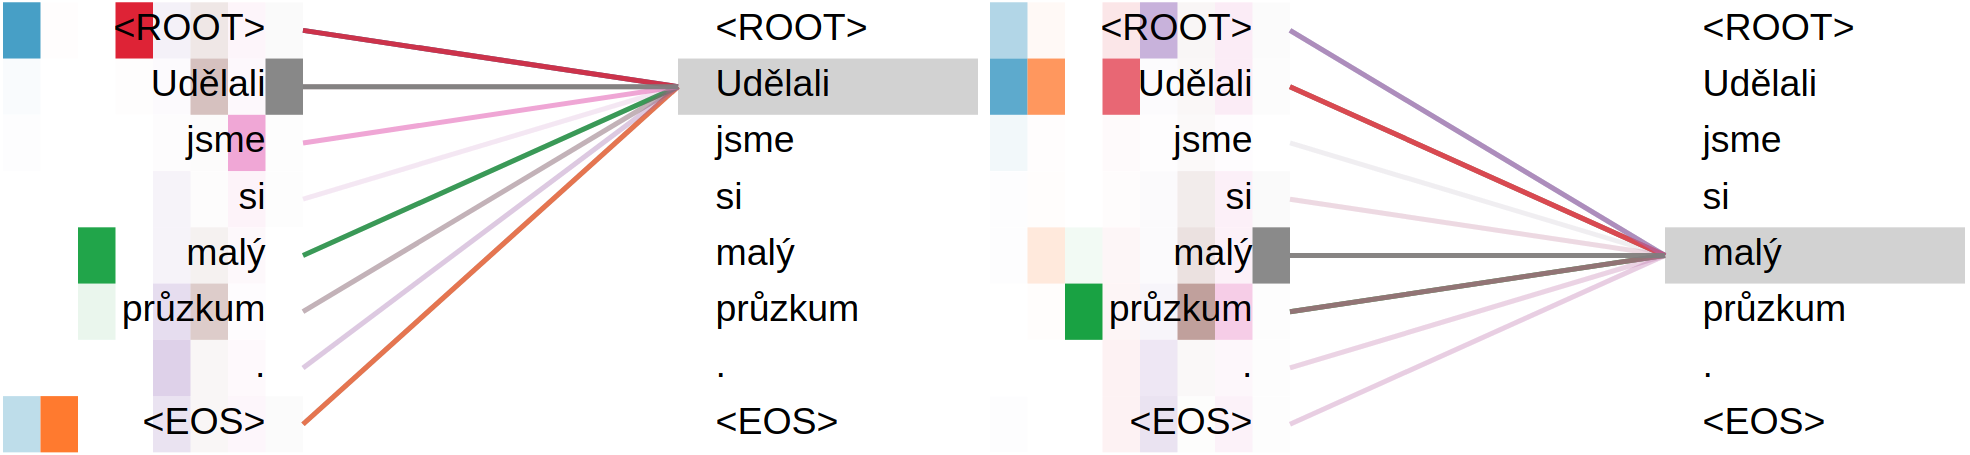
\includegraphics[width=\textwidth]{img/att-from4-l3.png}
        \caption{Layer 3}
    \end{subfigure}
    \par\medskip
    \begin{subfigure}[b]{0.9\textwidth}
        \centering
	    \frame{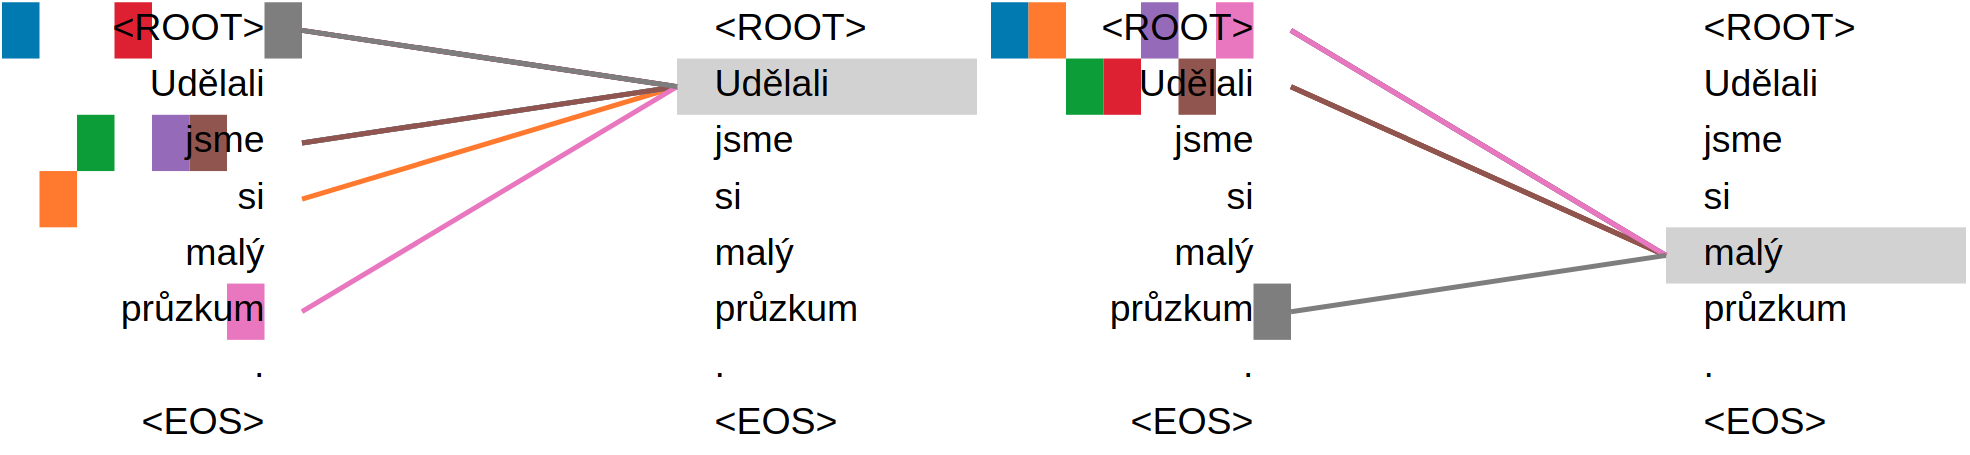
\includegraphics[width=\textwidth]{img/att-from4-l4.png}}
        \caption{Layer 4}
    \end{subfigure}
    \par\medskip
    \begin{subfigure}[b]{0.9\textwidth}
        \centering
	    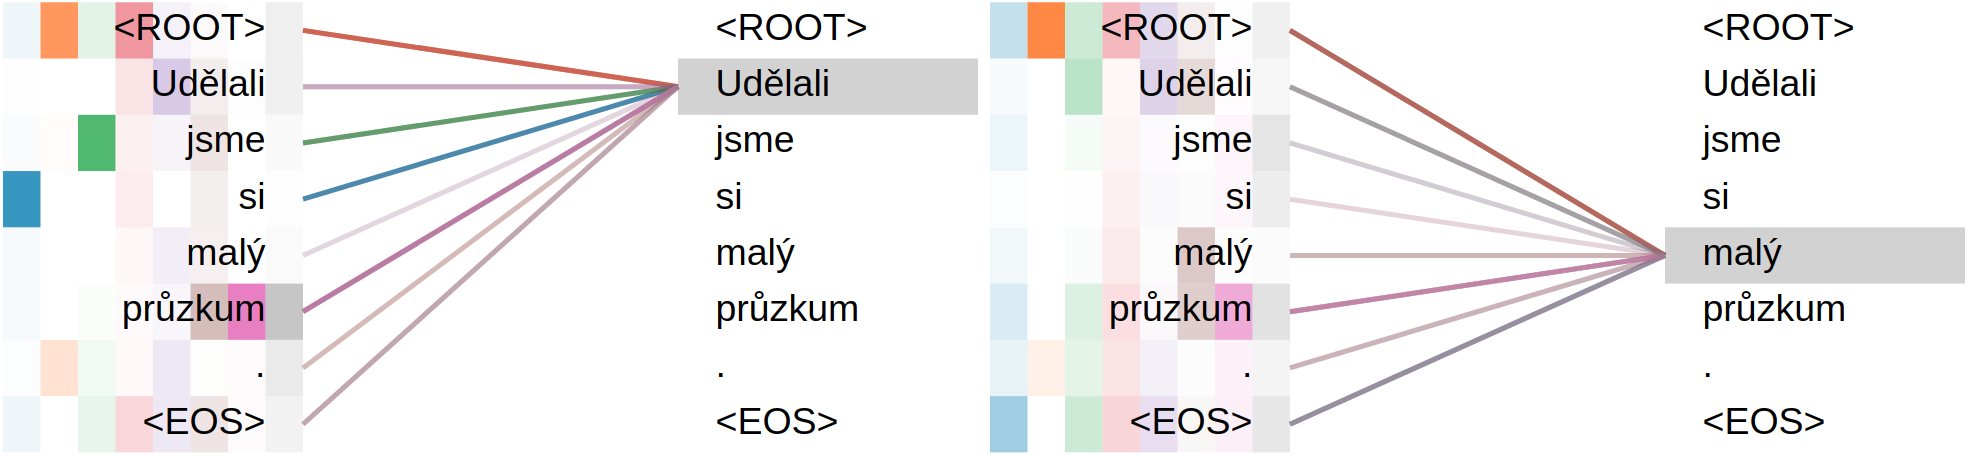
\includegraphics[width=\textwidth]{img/att-from4-l5.png}
        \caption{Layer 5}
    \end{subfigure}
    \caption{\DepParse model with syntax demanded from the encoder's layer 4, displaying more focused attention at that layer (framed).}
    \label{fig:att-from4}
\end{figure}


\section{Training Speed}
\label{result-speed}

\begin{figure}[t]
    \centering
    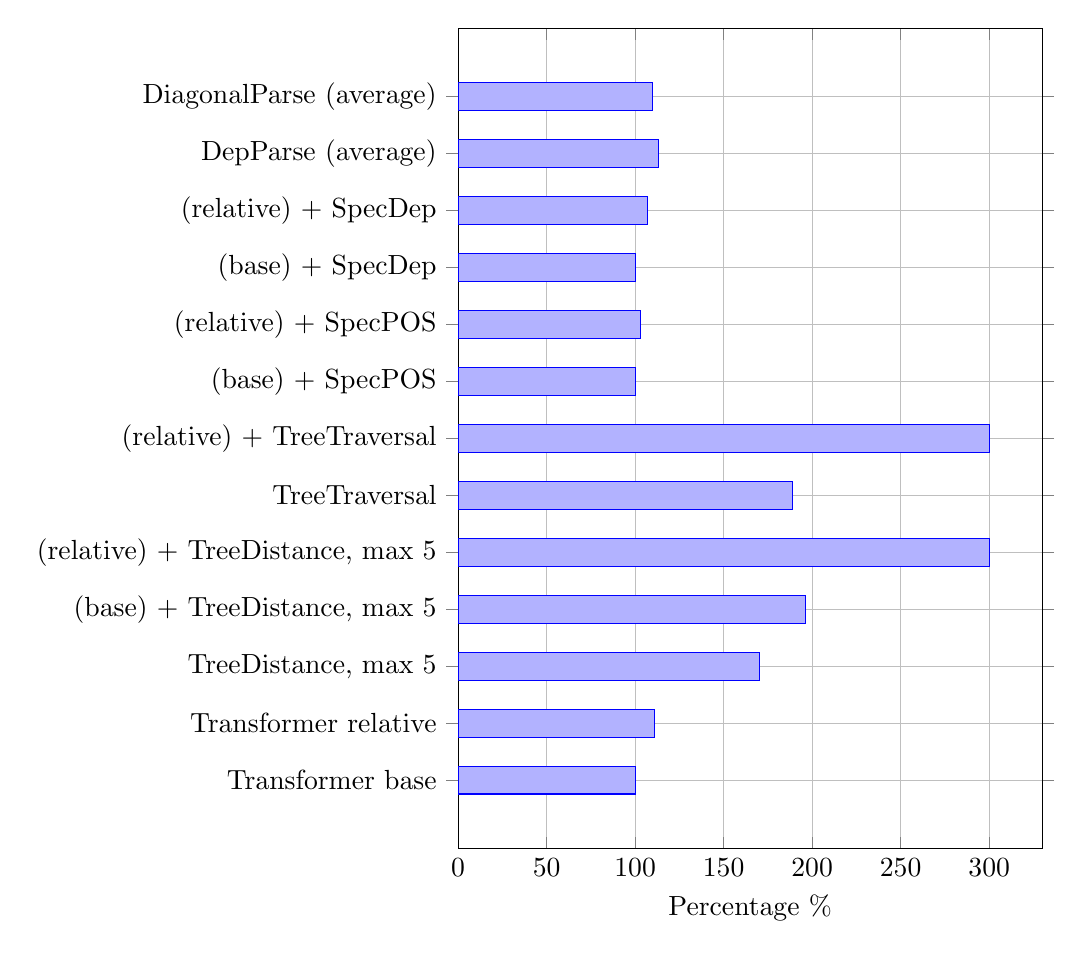
\begin{tikzpicture}
        \begin{axis}[
        height=12cm, width=9cm, grid=major,
        xbar, xmin=0,
        xlabel={Percentage \%},
        symbolic y coords={
            {Transformer base},
            {Transformer relative},
            {TreeDistance, max 5},
            {(base) + TreeDistance, max 5},
            {(relative) + TreeDistance, max 5},
            {TreeTraversal},
            {(relative) + TreeTraversal},
            {(base) + SpecPOS},
            {(relative) + SpecPOS},
            {(base) + SpecDep},
            {(relative) + SpecDep},
            {DepParse (average)},
            {DiagonalParse (average)}
        },
        ytick=data,
        % nodes near coords, nodes near coords align={horizontal},
        ytick=data,
        ]
        \addplot coordinates {
            (100,{Transformer base})
            (111,{Transformer relative})
            (170,{TreeDistance, max 5})
            (196,{(base) + TreeDistance, max 5})
            (300,{(relative) + TreeDistance, max 5})
            (189,{TreeTraversal})
            (300,{(relative) + TreeTraversal})
            (100,{(base) + SpecPOS})
            (103,{(relative) + SpecPOS})
            (100,{(base) + SpecDep})
            (107,{(relative) + SpecDep})
            (113,{DepParse (average)})
            (110,{DiagonalParse (average)})
        };
        \end{axis}
    \end{tikzpicture}
    \caption{Training time to reach 250,000 steps on a single GPU NVIDIA GTX 1080 Ti (relative to \transformerbase).}
    \label{fig:training-speed}
\end{figure}

Having documented that the \transformer NMT model has already captured dependency syntax, it is interesting to look at the training cost of the baseline and joint models.
Our joint models derived from the \transformer were trained in a comparable time with the single-task \transformerbase.

The training time (including internal evaluation every 1,000 steps) to reach 250,000 steps for the \transformerbase was 1 day, 3 hours, 48 minutes on a single GPU NVIDIA GTX 1080 Ti.
On average, our joint dependency parsing and translation model \DepParse took only 13\% longer than the \transformerbase with a significant improvement in the translation task. \cref{fig:training-speed} also reveals the same for joint diagonal parsing and translation model \DiagonalParse, which took 10\% more time to train than the \transformerbase.

The training times of encoder's enriched models with specialized attention heads are nearly identical to \transformerbase and \transformerrel.
The \SpecPOS models derived from \transformerbase and from \transformerrel took no extra time in comparison to those baselines.
This also applies to the \SpecDep models. 
However, they are different from the \SpecPOS models in that they brought considerable improvements.

While having achieved similar results in translation task, the other set of methods enriching the encoder consumed more time to train.
In detail, \TreeDistance with maximum distance of 5 consumed 70\% more of the time needed to train \transformerbase, while \TreeTraversal required 89\% more.
Combined with positional encoding, \TreeDistance max 5 took 96\% more time in training, but this cost brought significant improvements over both \transformerbase and \transformerrel.
Finally, the total training times for the \TreeDistance max 5 and the \TreeTraversal when combined with relative positions are both 300\% of the \transformerbase's training time (+200\%).
This huge amount of surplus training time was shown to yield improvements as well (\cref{result-enriching}).

The extra amount of training time required by the family of \TreeDistance and \TreeTraversal models were caused by the tree distance and tree encoding matrix's generation, and also the multiplication of these matrices with key and query vectors.
These computations are quadratic in the length of the input sentence and need to be done on every attention layer of the encoder.
Interestingly, the joint models consumed only a little more time than \transformerbase but brought improvements in translation tasks and a good parsing accuracy.
This result was possible thanks to the fact that our joint models do not add any separate parser on top of the encoders as the common practice in multi-task models, but use the self-attention matrix as the near output layer, then top it with an $argmax$ layer for the head selection.
